\chapter[Mix\&Slice]{Mix\&Slice:\\Efficient Access Revocation\\in the Cloud}\label{chap:ms}

We present an approach to enforce access revocation on resources stored at external cloud providers. The approach relies on a resource transformation that provides strong mutual inter-dependency in its encrypted representation. To revoke access on a resource, it is then sufficient to update a small portion of it, with the guarantee that the resource as a whole (and any portion of it) will become unintelligible to those from whom access is revoked. The extensive experimental evaluation on a variety of configurations confirmed the effectiveness and efficiency of our solution, which showed excellent performance and compatibility with several implementation strategies.

\section{Introduction}\label{ms:sec:intro}

With the considerable advancements in ICT solutions, users and companies are finding increasingly appealing to rely on external services for storing resources and making them available to others. In such contexts, a promising approach to enforce access control to externally stored resources is via encryption: resources are encrypted for storage and only authorized users have the keys that enable their decryption. There are several advantages that justify the use of encryption for enforcing access control. First, robust encryption has become computationally inexpensive, enabling its introduction in domains that are traditionally extremely sensitive to performance (like cloud-based applications and management of large resources). Second, encryption provides protection against the service provider itself, which - while trustworthy for providing access - cannot typically be considered authorized to know the content of the resources it stores ({\em honest-but-curious\/} scenario) and hence also to enforce access control. Third, encryption solves the need of having a trusted party for policy enforcement: resources enforce self-protection, since only authorized users, holding the keys, will be able to decrypt them.
 
One of the complex aspects in using encryption to enforce access control policy concerns access revocation. If granting an authorization is easy (it is sufficient to give the newly authorized user access to the key), revoking an authorization is a completely different problem. There are essentially two approaches to enforce revocation: {\em i)\/} re-encrypt the resource with a new key or {\em ii)\/} revoke access to the key itself. Re-encryption of the resource entails, for the data owner, downloading the resource, decrypting it and re-encrypting it with a new key, re-uploading the resource, and re-distributing the key to the users who still hold authorizations. If decryption, re-encryption, and even key management (for this specific context) can today be considered not an issue, the big problem is represented by the need of downloading and re-uploading the resource, with a considerable overhead for the data owner. This overhead, already an obstacle today, will become even more so in emerging big data contexts. The alternative approach of enforcing revocation on the resource by preventing access to the key with which the resource is encrypted cannot be considered a solution. As a matter of fact, it protects the key, not the resource itself, and it is inevitably fragile against a user who - while having been revoked from an access - has maintained a local copy of the key. Since keys are compact in size, such a threat is indeed real.

\medskip
\noindent{\bf Our approach.}
In this paper, we present a novel approach to enforce access revocation that provides efficiency, as it does not require expensive upload/re-upload of (large) resources, and robustness, as it is resilient against the threat of users who might have maintained copies of the keys protecting resources on which they have been revoked access.

The basic idea of our approach is to provide an encrypted representation of the resources that guarantees complete interdependence ({\em mixing\/}) among the bits of the encrypted content. Such a guarantee is ensured by using different rounds of encryption, while carefully selecting their input to provide complete mixing, meaning that the value of each bit in the resulting encrypted content depends on every bit of the original plaintext content. In this way, unavailability of even a small portion of the encrypted version of a resource completely prevents the reconstruction of the resource or even of portions of it. Brute-force attacks guessing possible values of the missing bits are possible, but even for small missing portions of the encrypted resource, the required effort would be prohibitive.
The {\em all-or-nothing transform} (AONT)~\cite{r97} considers similar requirements, but the techniques proposed for it are not suited to our scenario, because they are based on the assumption that keys are not known to users, whereas in our scenario revoked users can know the encryption key and may plan ahead to locally store critical pieces of information.

Trading off between the potentially clashing need of connecting all bits of a resource to provide the wished interdependency of the content on one side, and the potential huge size of the resources and need to maintain a possible fine-granularity of access within the resource itself on the other side, we apply the idea of mixing content within portions of the resource, enforcing then revocation by overwriting encrypted bits in every such portion. Before mixing, our approach partitions the resource in different, equally sized, chunks, called {\em macro-blocks\/}. Then, as the name hints, it is based on the following concepts.

\begin{itemize}

\item {\em Mix:\/} the content of each macro-block is processed by  an iterative application of different encryption rounds together with  a carefully designed bit mixing, that ensures, at the end of the process, that every individual bit in the input has had impact on each of the bits in the encrypted output.

\item {\em Slice:\/} the mixed macro-blocks are sliced into fragments so that  fragments provide complete coverage of the resource content and each fragment represents a minimal (in terms of number of bits of protection, which we call {\em mini-block\/}) unit of revocation: lack of any single fragment of the resource completely prevents reconstruction of the resource or of portions of it.
\end{itemize}

To revoke access from a user, it is sufficient to re-encrypt one (any one) of the resource fragments with a new key not known to the user. The advantage is clear: re-encrypting a tiny chunk of the resource guarantees protection of the whole resource itself. Also, the cloud provider simply needs to provide storage functionality and is not required to play an active role for enforcing access control or providing user authentication. Our \name\ proposal is complemented with a convenient approach for key management that, based on key regression, avoids any storage overhead for key distribution.

\medskip
\noindent{\bf Outline.}
The remainder of the paper is organized as follows. Section~\ref{ms:sec:mixslice} illustrates our approach to produce an encrypted representation with the desired guarantees. Section~\ref{ms:sec:revoke} presents the enforcement of access revocation. Section~\ref{ms:sec:security} discusses the effectiveness of our solution in providing revocation. Section~\ref{ms:sec:expe} illustrates our implementation and the extensive experimental evaluation confirming its advantages and applicability. Section~\ref{ms:sec:relwork} discusses related work. Finally, Section~\ref{ms:sec:conclu} presents our conclusions.

% ------

\section{Mix \& Slice}\label{ms:sec:mixslice}

\subsection{Blocks, mini-blocks, and macro-blocks}

The basic building block of our approach is the application of a symmetric block cipher. A symmetric cryptographic function operating on blocks guarantees complete dependency of the encrypted result from every bit of the input and the impossibility, when missing some bits of an encrypted version of a block, to retrieve the original plaintext block (even if parts of it are known). The only possibility to retrieve the original block would be to perform a brute-force attack attempting all the possible combinations of values for the missing bits. For instance, modern encryption functions like AES guarantee that the absence of $i$ bits from the input (plaintext) and of $o$ bits from the output (ciphertext) does not permit, even with knowledge of the encryption key \key{}, to properly reconstruct the plaintext and/or ciphertext, apart from performing a brute-force attack generating and verifying all the $2^{{\rm min}(i,o)}$ possible configurations for the missing bits~\cite{abm14}.

Clearly, the larger the number of bits that are missing in the encrypted version of a block, the harder the effort required to perform a brute-force attack, which requires attempting $2^x$ possible combinations of values when $x$ bits are missing. Such {\em security parameter\/} is at the center of our approach and we explicitly identify a sequence of bits of its length as the atomic unit on which our approach operates, which we call {\em mini-block\/}. Applying block encryption with explicit consideration of such atomic unit of protection, and extending it to a coarser-grain with iterative rounds, our approach identifies the following basic concepts.

\begin{itemize}

\item {\em Block\/}: a sequence of bits input to a
  block cipher (it corresponds to the classical block concept).

\item {\em Mini-block\/}: a sequence of bits, of a specified length,
  contained in a block. It represents our {\em atomic unit\/} of
  protection (i.e., when removing bits, we will operate at the
  level of mini-block removing all its bits).

\item {\em Macro-block\/}: a sequence of blocks. It allows extending
  the application of block cipher on sequences of bits larger than
  individual blocks. In particular, our approach operates {\em
    mixing\/} bits at the macro-block level, extending protection to
  work against attacks beyond the individual block.

\end{itemize}

Our approach is completely parametric with respect to the size (in terms of the number of bits) that can be considered for blocks, mini-blocks, and macro-blocks. The only constraints are for the size of a mini-block to be a divisor of the size of the block (aspect on which we will elaborate later on) and for the size of a macro-block to be a product of the size of a mini-block and a power of the number of mini-blocks in a block (i.e., the ratio between the size of a block and the size of a mini-block). In the following, for concreteness and simplicity of the figures, we will illustrate our examples assuming the application of AES with blocks of 128 bits and mini-blocks of 32 bits, which corresponds to having 4 mini-blocks in every block and therefore operating on macro-blocks of size $32 \cdot 4^x$, with $x$ arbitrarily set. In the following, we will use \msize, \bsize, \Msize\ to denote the size (in bits) of mini-blocks, blocks, and macro-blocks, respectively. We will use $b_j[i]$ (\macroblock{j}$[i]$, resp.) to denote the $i$-th mini-block in a block $b_j$ (macro-block \macroblock{j}, resp.). We will simply use notation $[i]$ to denote the $i$-th mini-block in a generic bit sequence (be it a block or macro-block), and $[[j]]$ to denote the $j$-th block. In the encryption process, a subscript associated with a mini-block/block denotes the round that produced it.

\begin{figure}[!t]
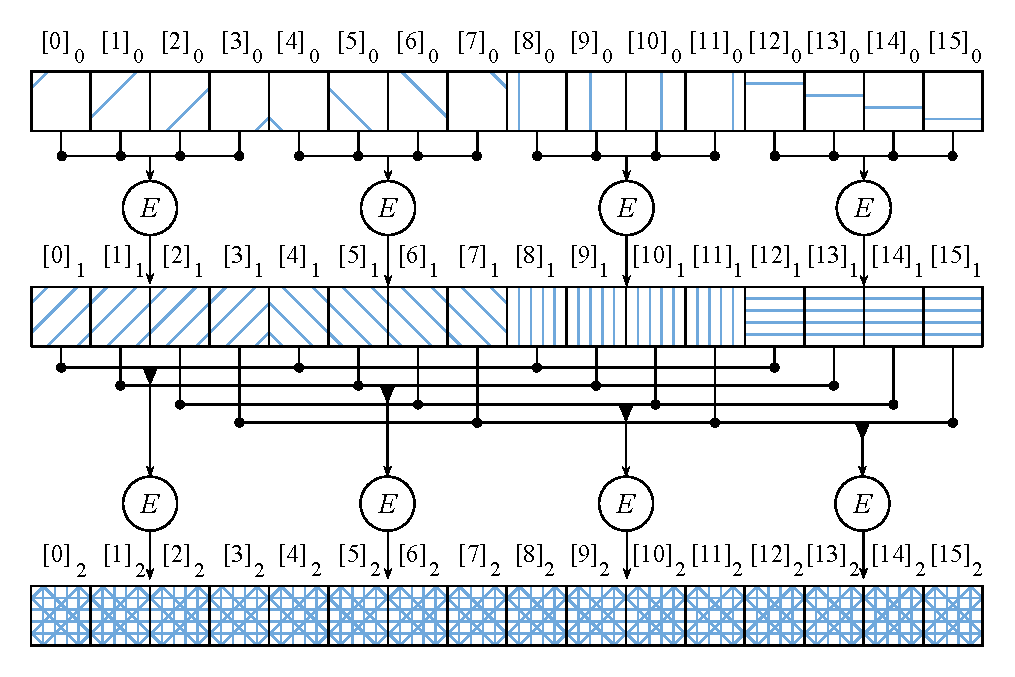
\includegraphics[width=\columnwidth]{chapters/ms/figures/fig01.eps}\\
\vspace*{-0.7cm}
\caption{\label{ms:fig:mixing} An example of mixing of 16 mini-blocks assuming $m=4$}
\end{figure}

\subsection{Mixing}

The basic step of our approach (on which we will iteratively build to provide complete mixing within a macro-block) is the application of encryption at the block level. This application is visible at the top of Figure~\ref{ms:fig:mixing}, where the first row reports a sequence of 16 mini-blocks ($[0],\ldots,[15]$) composing 4 blocks. The second row is the result of block encryption on the sequence of mini-blocks. As visible from the pattern-coding in the figure, encryption provides mixing within each block so that each mini-block in the result is dependent on every mini-block in the same input block. In other words, each $[i]_1$ is dependent on every $[j]_0$ with ($i$ \mydiv 4) = ($j$ \mydiv 4).

One round of block encryption provides mixing only at the level of block. With reference to our example, mixing is provided among mini-blocks $[0]_0 \ldots [3]_0$, $[4]_0 \ldots [7]_0$, $[8]_0 \ldots [11]_0$, and $[12]_0 \ldots [15]_0$, respectively. Absence of a mini-block from the result will prevent reconstruction only of the plaintext block including it, while not preventing the reconstruction of all the other blocks. For instance, with reference to our example, absence of $[0]_1$ will prevent reconstruction of the first block (mini-blocks $[0]_0, \ldots, [3]_0$) but will not prevent reconstruction of the other three blocks (mini-blocks $[4]_0, \ldots, [15]_0$). Protection at the block level is clearly not sufficient in our context, where we expect to manage resources of arbitrarily large size and would like to provide the guarantee that the lack of any individual mini-block would imply the impossibly (apart from performing a brute-force attack) of reconstructing any other mini-block of the resource. The concept of macro-block, and accurate extension of block ciphering to operate across blocks, allows us to provide mixing on an arbitrarily long sequence of bits (going much above the size of the block).

The idea is to extend mixing to the whole macro-block by the iterative application of block encryption on, at each round, blocks composed of mini-blocks that are representative (i.e., belong to the result) of different encryptions in the previous round. Before giving the general definition of our approach, let us discuss the simple example of two rounds illustrated in Figure~\ref{ms:fig:mixing}, where $[0]_1, \ldots, [15]_1$ are the mini-blocks resulting from the first round. The second round would apply again block encryption, considering different blocks each composed of a representative of a different computation in the first round. To guarantee such a composition, we define the blocks input to the four encryption operations as composed of mini-blocks that are at distance 4 (=\mnumb) in the sequence, which corresponds to say that they resulted from different encryption operations in the previous round. The blocks considered for encryption would then be $\langle [0]_1[4]_1[8]_1[12]_1\rangle,$ $\langle [1]_1[5]_1[9]_1[13]_1\rangle,$$ \langle [2]_1[6]_1[10]_1[14]_1\rangle, $$\langle [3]_1[7]_1[11]_1[15]_1 \rangle.$ The result would be a sequence of 16 mini-blocks, each of which is dependent on each of the 16 original mini-blocks, that is, the result provides mixing among all 16 mini-blocks, as visible from the pattern-coding in the figure. With 16 mini-blocks, two rounds of encryption suffice for guaranteeing mixing among all of them. Providing mixing for larger sequences clearly requires more rounds. This brings us to the general formulation of our approach operating at the level of macro-block of arbitrarily large size (the example just illustrated being a macro-block of 16 mini-blocks).

To ensure the possibility of mixing, at each round, blocks composed of mini-blocks resulting from different encryption operations of the previous round, we assume a macro-block composed of a number of mini-blocks, which is the power of the number (\mnumb) of mini-blocks in a block. For instance, with reference to our running example where blocks are composed of 4 mini-blocks (i.e., \mnumb=4), macro-blocks can be composed of $4^x$ mini-blocks, with an arbitrary $x$ ($x$=2 in the example of Figure~\ref{ms:fig:mixing}). The assumption can be equivalently stated in terms of blocks, where the number of blocks \bnum\ will be $4^{x-1}$. Any classical padding solution can be employed to guarantee such a requirement, if not already satisfied by the original bit sequence in input.

\begin{figure}[!t]
\begin{scriptsize}
\hrule          %
\vspace{0.12cm}
\begin{tabbing}
{\bf Mix}(\macroblock{})\\   
\num{1:~}\= \myfor\ $i:= 1, \ldots, x$ \com{do} \comm{at each round $i$}\\
\num{2:~}\2 \spanna\ := \mnumb$^i$  \comm{number of mini-blocks in a mixing}\\
\num{3:~}\2 \distance\ := \mnumb$^{i -1}$ \comm{leg of mini-blocks input to an encryption}\\
\num{4:~}\2 \myfor\ $j:= 0, \ldots, \bnum -1$ \com{do} \comm{each $j$ is an encryption}\\
             \3 \comm{identify the input to the $j$-th encryption picking,}\\
             \3 \comm{within each span, mini-blocks at leg \distance}\\
\num{5:~}\3 let \= {\em block} be the concatenation of all mini-blocks $[l]$\\
\num{6:~}\4 s.t.\= \ $(l\mod\distance) = j$ and  \\
\num{7:~}\5 ($j \cdot \mnumb$) \mydiv \spanna\ = $l$ \mydiv \spanna\\
\num{8:~}\3 $[[j]]_i := E(k,block)$ \comm{write the result as the $j$-th block in output}
\end{tabbing}
\vspace{-0.3cm}
\hrule
\end{scriptsize}
\caption{\label{ms:fig:encrypt}Mixing within a macro-block \macroblock{}}
\end{figure}

\begin{figure*}[!t]
\begin{center}
{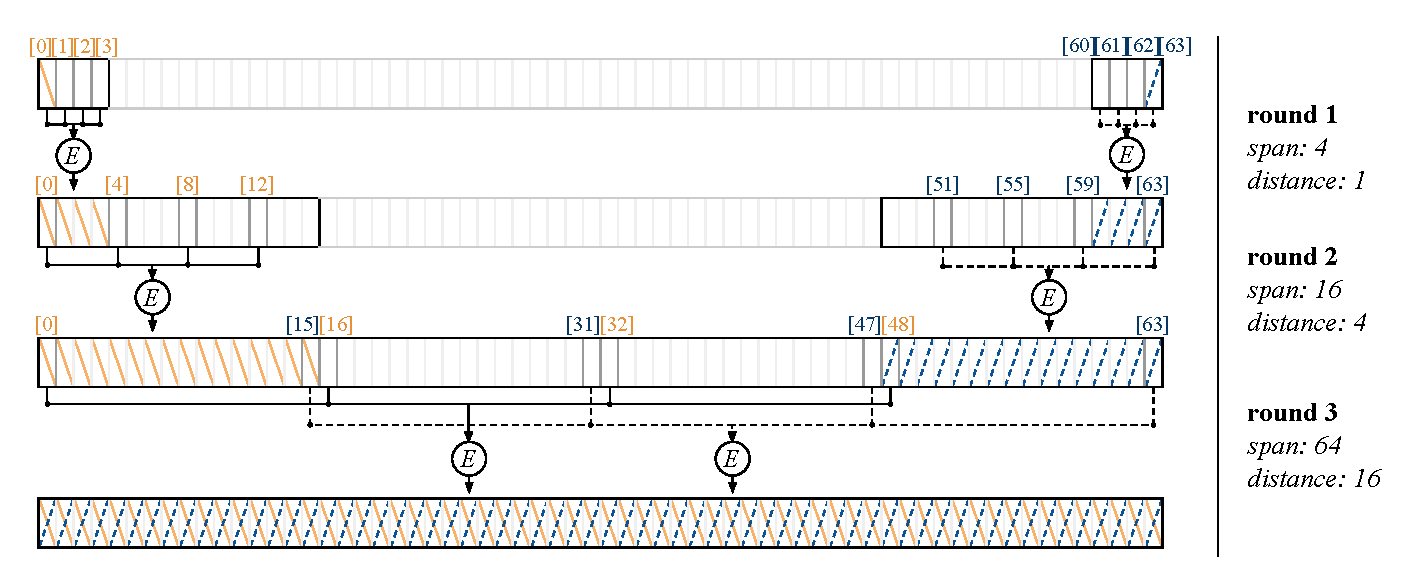
\includegraphics[width=0.85\textwidth]{chapters/ms/fig03.eps}}\\
\vspace*{-0.6cm}
\end{center}
\caption{\label{ms:fig:general}Propagation of the content of mini-blocks [0] and [63] in the mix process}
\end{figure*}

Providing mixing of a macro-block composed of \bnum\ blocks with \bnum=\mnumb$^{x-1}$ requires $x$ rounds of encryption each composed of \bnum\ encryptions. Each round allows mixing among a number \spanna\ of mini-blocks that multiplies by \mnumb\ at every round. At round $i$, each encryption $j$ takes as input \mnumb\ mini-blocks that are within the same \spanna\ (i.e., the same group of $\mnumb^i$ mini-blocks to be mixed) and at a \distance\ ($\mnumb^{i-1}$). Figure~\ref{ms:fig:encrypt} illustrates the mixing procedure. To illustrate, consider the example in Figure~\ref{ms:fig:mixing}, where blocks are composed of 4 mini-blocks (\mnumb=4) and we have a macro-block of 16 mini-blocks, that is, 4 blocks (\bnum=4). Mixing requires $x=2$ rounds of encryption ($16=4^2$), each composed of 4 (\bnum) encryptions operating on 4 (\mnumb) mini-blocks. At round 1, the \spanna\ is 4 (i.e., mixing operates on chunks of 4 mini-blocks) and mini-blocks input to an encryption are taken at distance 1 within each span. At round 2, the \spanna\ is 16 (all mini-blocks are mixed) and mini-blocks input to an encryption are taken at \distance\ 4 within each \spanna. Let us consider, as an another example, a macro-block composed of 64 mini-blocks (i.e., 16 blocks). Mixing requires 3 rounds. The first two rounds would work as before, with the second round producing mixing within chunks of 16 mini-blocks. The third round would then consider a \spanna\ of all the 64 mini-blocks and mini-blocks input to an encryption would be the ones at \distance\ 16.

At each round $i$, mini-blocks are mixed among chunks of $\mnumb^i$ mini-blocks, hence ensuring at round $x$, mixing of the whole macro-block composed of $\mnumb^x$ mini-blocks.

Figure~\ref{ms:fig:general} captures this concept by showing the mixing of the content of the first ([0]) and last ([63]) mini-blocks of the macro-block at the different rounds, given by the encryption to which they (and those mini-blocks mixed with them in previous rounds) are input, showing also how the two meet at the step that completes the mixing. While for simplicity the figure pictures only propagation of the content of two mini-blocks, note that at any step they (just like other mini-blocks) actually carry along the content of all the mini-blocks with which they mixed in previous rounds. Given a macro-block \macroblock{} with \mnumb$^x$ mini-blocks (corresponding to \bnum\ blocks), the following two properties hold: {\em 1)\/} a generic pair of mini-blocks $[i]$ and $[j]$ mix at round $r$ with $i$ \mydiv\ \mnumb$^r$ = $j$ \mydiv\ \mnumb$^r$; and {\em 2)\/} $x$ rounds bring complete mixing. In other words, the number of encryption rounds needed to mix a macro-block with $\mnumb \cdot \bnum$ mini-blocks is $\log_{\mnumb}(\mnumb\cdot\bnum)$.

An important feature of the mixing is that the number of bits that are passed from each block in a round to each block in the next round is equal to the size of the mini-block. This guarantees that the uncertainty introduced by the absence of a mini-block at the first round ($2^{\msize}$) maps to the same level of uncertainty for each of the blocks involved in the second round, and iteratively to the next rounds, thanks to the use of AES at each iteration. This implies that a complete mixing of the macro-block requires at least  $\log_{\mnumb} (\mnumb \cdot \bnum)$ rounds, that is, the rounds requested by  our technique.

Another crucial aspect is that the representation after each round has to be of the same size as the original macro-block. In fact, if the transformation produced a more compact representation, there would be a possibility for a user to store this compact representation and maintain access to the resource even after revocation (this is a weakness of other solutions discussed in Section~\ref{ms:sec:relwork}). Since, in our approach, each round produces a representation that has the same macro-block size, the user has no benefit in aiming to attack one round compared to another (see Section~\ref{ms:sec:security}).

We note that an interpretation of the proposed mixing is that it extends the ability of protecting the correspondence between input and output of a block cipher to blocks of arbitrary size. An alternative approach that we considered to obtain this result was based on the use of a Feistel architecture~\cite{lr88}, which is known to be an effective technique for the construction of block ciphers. The approach uses, as the {\em round} function of the Feistel architecture, a block cipher. The approach can be applied iteratively, doubling the block size at every iteration. The analysis we performed showed that this approach would lead to less efficiency compared to the solution proposed in this paper, with a number of invocations of the basic block cipher equal to $2\cdot \log_{\mnumb} (\mnumb \cdot \bnum)$. The Feistel-based approach can be adopted when the mini-block size desired for security goes beyond the block size of the available block cipher. Similarly, symmetric cryptosystems operating on large blocks can support larger mini-blocks and also reduce the number of rounds of our approach. For instance,  AESQ~\cite{paeq,paeq2} shuffles 4 AES blocks and could be used as a 512-block cipher in our structure.

When resources are extremely large (or when access to a resource involves only a portion of it) considering a whole resource as a single macro-block may be not desirable. Even if only with a logarithmic dependence, the larger the macro-block the more the encryption (and therefore decryption to retrieve the plaintext) rounds required. Also, encrypting the whole resource as a single macro-block implies its complete download at every access, when this might actually not be needed for service.

Accounting for this, we do not assume a resource to correspond to an individual macro-block, but assume instead that any resource can be partitioned into \Mnum\ macro-blocks, which can then be mixed independently. The choice of the size of macro-blocks should take into consideration the performance requirements of both the data owner (for encryption) and of clients (for decryption), and the possible need to serve fine-grained retrieval of content. This requirement can be then efficiently accommodated independently encrypting (i.e., mixing) different portions of the resource, which can be downloaded and processed independently (we will discuss this in Section~\ref{ms:sec:overlay}).

Encryption of a resource would then entail a preliminary step cutting the resource in different, equally sized, macro-blocks on which mixing operates. To ensure the mixed versions of macro-blocks be all different, even if with the same original content, the first block of every macro-block is {\sc xor}ed with an {\em initialization vector\/} (\var{IV}) before starting the mixing process. Since mixing guarantees that every block in a macro-block influences every other block, the adoption of a different initialization vector for each macro-block guarantees indistinguishability among their encrypted content. The different initialization vectors for the different blocks can be obtained by randomly generating a vector for the first macro-block and then incrementing it by 1 for each of the subsequent macro-blocks in the resource, in a way similar to the CTR mode~\cite{d01}. Figure~\ref{ms:fig:mixslice}(a) illustrates such process.

\begin{figure}[!t]
{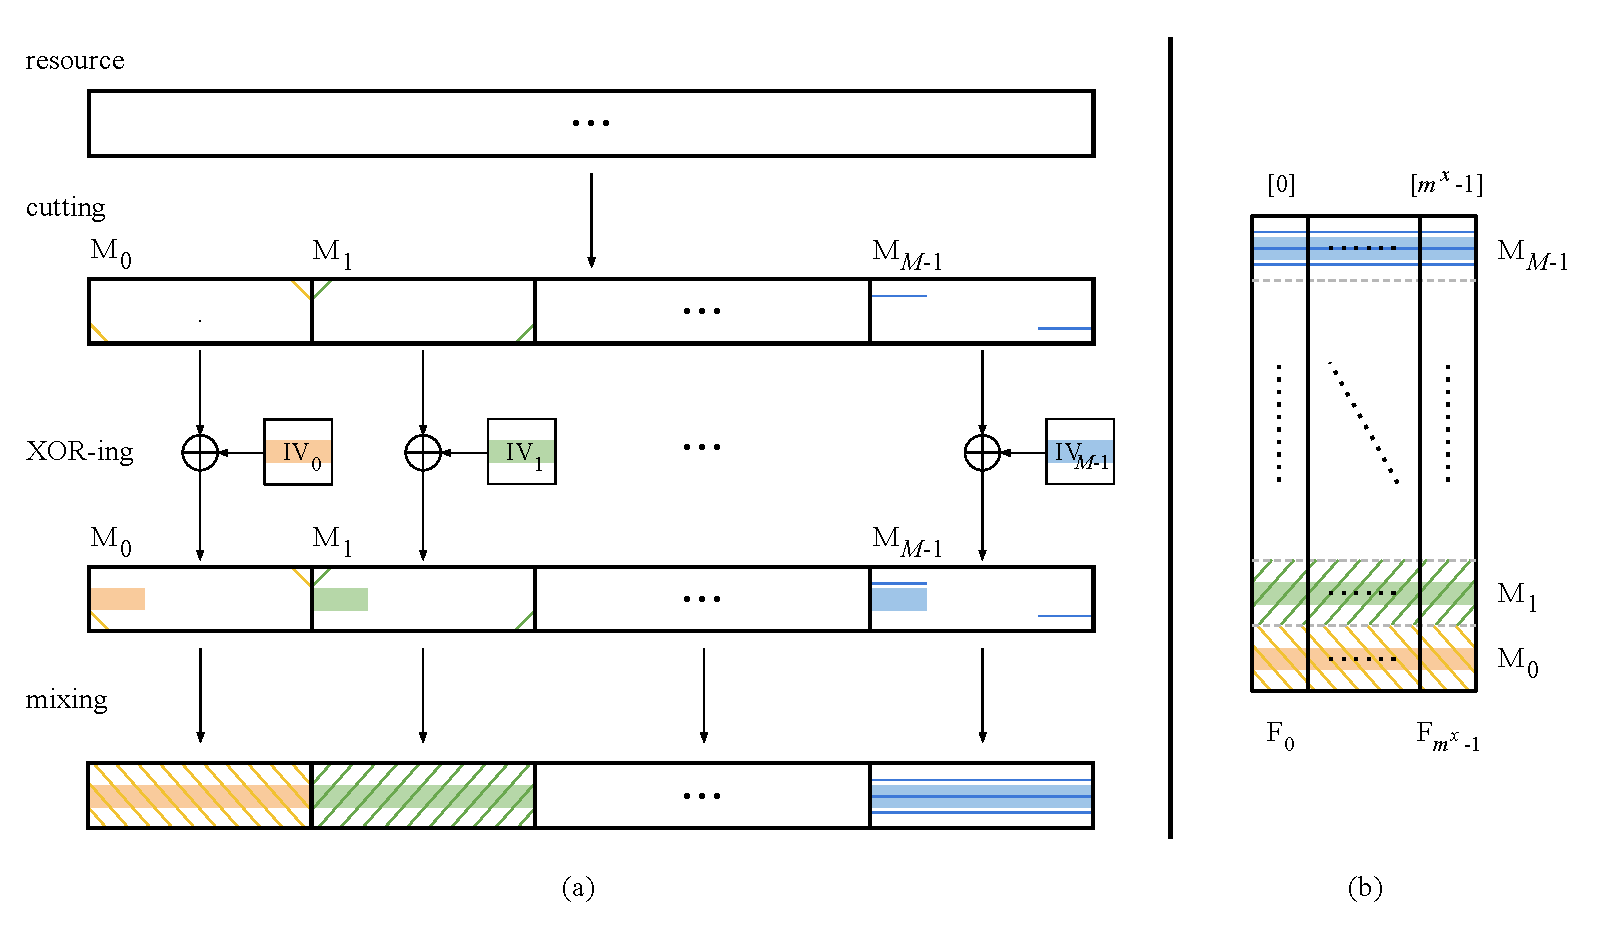
\includegraphics[width=\columnwidth]{chapters/ms/fig04.eps}}\\
\vspace*{-0.3cm}
\caption{\label{ms:fig:mixslice} From resource to fragments}
\end{figure}

\subsection{Slicing}

The starting point for introducing mixing is to ensure that each single bit in the encrypted version of a macro-block depends on every other bit of its plaintext representation, and therefore that removing any one of the bits of the encrypted macro-block would make it impossible (apart from brute-force attacks) to reconstruct any portion of the plaintext macro-block. Such a property operates at the level of macro-block. Hence, if a resource (because of size or need of efficient fine-grained access) has been partitioned into different macro-blocks, removal of a mini-block would only guarantee protection of the macro-block to which it belongs, while not preventing reconstruction of the other macro-blocks (and therefore partial reconstructions of the resource). Resource protection can be achieved if, for each macro-block of which the resource is composed, a mini-block is removed. This observation brings to the second concept giving the name to our approach, which is {\em slicing}. Slicing the encrypted resource consists in defining different {\em fragments} such that a fragment contains a mini-block for each macro-block of the resource, no two fragments contain the same mini-block, and for every mini-block there is a fragment that contains it. To ensure all this, as well as to simplify management, we slice the resource simply putting in the same fragment the mini-blocks that occur at the same position in the different macro-blocks. Slicing and fragments are defined as follows.

\begin{dfn}[Slicing and fragments]
Let \resource\ be a resource and $\macroblock{0},\ldots,\macroblock{\Mnum-1}$ be its (individually mixed) macro-blocks, each composed of $(\mnumb \cdot \bnum)$ mini-blocks. Slicing produces $(\mnumb \cdot \bnum)$ fragments for \resource\ where $\fragment{\var{i}}{}=\langle\miniinmacro{0}{\var{i}},\ldots,\miniinmacro{\Mnum-1}{\var{i}}\rangle$, with $i=1,\ldots,(\mnumb \cdot \bnum)$.
\end{dfn}

Figure~\ref{ms:fig:mixslice}(b) illustrates the slicing process and Figure~\ref{ms:fig:algoenc} illustrates the procedure for encrypting a resource \resource. \resource\ is first cut into \Mnum\ macro-blocks and an initialization vector is randomly chosen. The first block of each macro-block is then {\sc xor}-ed with the initialization vector, which is incremented by 1 for each macro-block. The macro-block is then encrypted with a mixing process (Figure~\ref{ms:fig:encrypt}). Encrypted macro-blocks are finally sliced into fragments.

% ------

\section{Access management}\label{ms:sec:revoke}

Accessing a resource (or a macro-block in the resource, resp.) requires availability of all its fragments (its mini-blocks in all the fragments, resp.), and of the key used for encryption. Policy changes corresponding to granting access to new users can be simply enforced, as usual, by giving them the encryption key. In principle, policy changes corresponding to revocation of access would instead normally entail downloading the resource, re-encrypting it with a new key, re-uploading the resource, and distributing the new encryption key to all the users who still hold authorizations. Our approach permits to enforce revocation of access to a resource by simply making any of its fragments unavailable to the users from whom the access is revoked. Since lack of a fragment implies lack of a mini-block for each macro-block of a resource, and lack of a mini-block prevents reconstruction of the whole macro-block, lack of a fragment equates to complete inability, for the revoked users, to reconstruct the plaintext resource or any portion of it. In other words, it equates to revocation.

\begin{figure}[!t]
\begin{scriptsize}
\hrule          %
\vspace{0.12cm}
\begin{tabbing}
{\bf Encrypt}\\ 
\num{1:~}\= cut \resource\ in $\Mnum$ macro-blocks $\macroblock{0},\ldots,\macroblock{\Mnum-1}$\\
\num{2:~}\1 apply padding to the last macro-block \macroblock{\Mnum-1}\\
\num{3:~}\1 \var{IV} := randomly choose an initialization vector\\
\num{4:~}\1 \myfor\ $i=0,\ldots,\Mnum-1$ \com{do} \comm{encrypt macro-blocks}\\
\num{5:~}\2     \macroblock{\var{i}}$[[1]]$ := \macroblock{\var{i}}$[[1]]$ $\oplus$ \var{IV} \comm{{\sc xor} the first block with the IV}\\
\num{6:~}\2     {\bf Mix}(\macroblock{\var{i}}) \comm{encrypt the macro-block}\\
\num{7:~}\2     \var{IV} := \var{IV} $+$ 1 \comm{initialization vector for the next macro-block}\\
\num{8:~}\2     \myfor\ $j=0,\ldots,\mnumb^x-1$ \com{do} \comm{slicing}\\
\num{9:~}\3         \fragment{\var{j}}{}[\var{i}] := \macroblock{\var{i}}$[j]$
\end{tabbing}
\vspace{-0.3cm}
\hrule
\end{scriptsize}
\caption{\label{ms:fig:algoenc}Algorithm for encrypting a resource \resource}
\end{figure}

\begin{figure*}[!t]
\setlength{\tabcolsep}{0.01cm}
\begin{tabular}{cc}
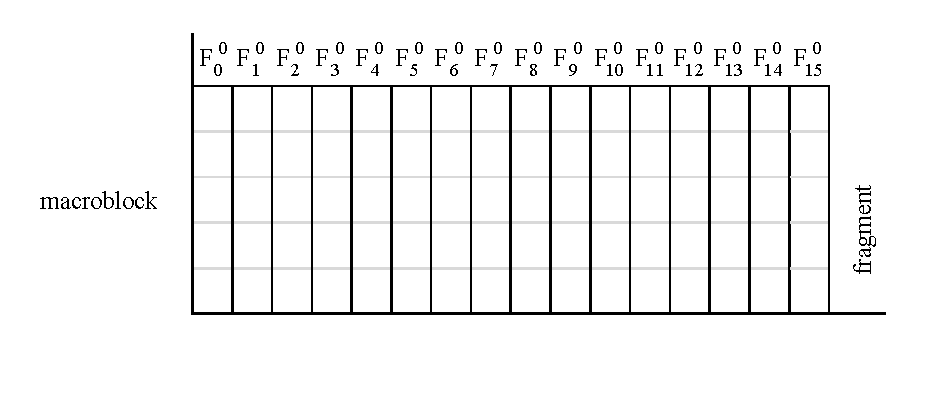
\includegraphics[width=.5\textwidth,valign=t]{chapters/ms/fig06a}&
\includegraphics[width=.5\textwidth,valign=t]{chapters/ms/fig06b}\\
{\scriptsize (a)} & {\scriptsize (b)} \\
\includegraphics[width=.5\textwidth,valign=t]{chapters/ms/fig06c}&
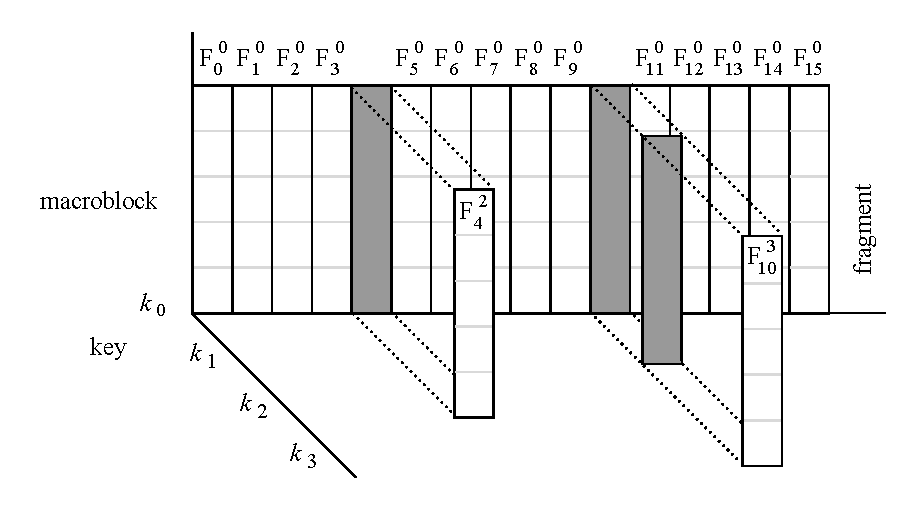
\includegraphics[width=.5\textwidth,valign=t]{chapters/ms/fig06d}\\
{\scriptsize (c)} & {\scriptsize (d)}\\
\end{tabular}
\caption{\label{ms:fig:pu}An example of fragments evolution}
\end{figure*}

Access revocations are then enforced by the data owner by randomly picking a fragment, which is then downloaded, re-encrypted with a new key (which will be made known only to users still authorized for the access), and re-uploaded at the server overwriting its previous version. While still requesting some download/re-upload, operating on a fragment clearly brings large advantages (in terms of throughput) with respect to operating on the whole resource (see Section~\ref{ms:sec:expe}). Revocation can be enforced on any randomly picked fragment (even if already re-written in a previous revocation) and a fresh new key is employed at every revoke operation. Figure~\ref{ms:fig:pu} illustrates an example of fragments evolution due to the enforcement of a sequence of revoke operations. Figure~\ref{ms:fig:pu}(a) is the starting situation with the original fragments computed as illustrated in Section~\ref{ms:sec:mixslice}. Figure~\ref{ms:fig:pu}(b-d) is the sequence of rewriting to enforce revocations, which involve, respectively, fragment \fragment{10}{}, re-encrypted with key \key{1}, fragment \fragment{4}{}, re-encrypted with key \key{2}, and fragment \fragment{10}{} again, now re-encrypted with key \key{3}. In the following, we use notation \fragment{\var{i}}{\var{j}} to denote a version of fragment \fragment{\var{i}}{} encrypted with key \key{j}, being \fragment{\var{i}}{0} the version of the fragment obtained through the mixing process. In the figure, the resource is represented in a three-dimensional space, with axes corresponding to fragments, macro-blocks, and keys. The re-writing of a fragment is represented by placing it in correspondence to the new key used for its encryption. The shadowing in correspondence to the previous versions of the fragments denote the fact that they are not available anymore as they are overwritten by the new versions.

Each revoke operation requires the use of a fresh new key and, due to policy changes, fragments of a resource might be encrypted with different keys. Such a situation does not cause any complication for key management, which can be conveniently and efficiently handled with a {\em key regression\/} technique~\cite{fkk06}. Key regression is an RSA-based cryptographically strong technique (the generated keys appear as pseudorandom) allowing a data owner to generate, starting from a seed \seed{0}, an unlimited sequence of symmetric keys $\key{0},\ldots,\key{u}$, so that simple knowledge of a key \key{i} (or the compact secret seed \seed{i} of constant size related to it) permits to efficiently derive all keys \key{j} with $j\leq i$. Only the data owner (who knows the private key used for generation) can perform forward derivation, that is, from \key{i}, derive keys following it in the sequence (i.e., \key{z} with $z\geq i$). Note instead that, not knowing the private key, users cannot perform forward derivation. The cost that users must pay for key derivation is small. On a single core, the computer we used for the experiments is able to process several hundred thousand key derivations per second.

With key regression, every user authorized to access a resource just needs to know the seed corresponding to the most recent key used for it (\seed{0} if the policy has not changed, \seed{3} in the example of Figure~\ref{ms:fig:pu}(d)). To this end, there is no need for key distribution, rather, such a seed can be stored in the resource descriptor and protected (encrypted) with a key corresponding to the resource's {\em acl\/} (i.e., known or derivable by all authorized users)~\cite{afb05,vldb07}. Enforcing revocation entails then, besides re-encrypting a randomly picked fragment with a fresh new key \key{i}, rewriting its corresponding seed \seed{i}, encrypted with a key associated with the new {\em acl\/} of the resource. Figure~\ref{ms:fig:revoke} illustrates the revocation process.

To access a resource, a user then first downloads the resource descriptor, to retrieve the most recent seed \seed{l}, and all the fragments. With the seed, she computes the keys necessary to decrypt fragments that have been overwritten, to retrieve their version encrypted with \key{0}. Then, she combines the mini-blocks in fragments to reconstruct the macro-blocks in the resource. She then applies mixing in decrypt mode to macro-blocks to retrieve the plaintext resource. Figure~\ref{ms:fig:access} illustrates the process to access a resource. 

Note that the size of macro-blocks influences the performance of both revoke and access operations. Larger macro-blocks naturally provide greater policy update performance as they decrease policy update cost linearly, with limited impact on the efficiency of decryption, since its cost increases logarithmically (Section~\ref{ms:sec:expe}).

% ------

\section{Effectiveness of the approach}\label{ms:sec:security}

In this section, we elaborate on the effectiveness of our approach for enforcing revocation. For the discussion, we recall that \msize\ is the size of individual mini-blocks, \mnumb\ is the number of mini-blocks in a block, \bnum\ is the number of blocks in a macro-block, and \Mnum\ is the number of macro-blocks. Also, we denote with \fnum\ \! the number of fragments, that is, $\fnum=\mnumb \cdot \bnum$.

We consider the threat coming from a user whose access to the resource has been revoked, and who downloads the resource from the server. With access policy enforced by encryption, not being authorized for an access should not prevent downloading the resource but rather it should prevent reconstruction of its plaintext representation. We then evaluate the protection against the user's attempts to reconstruct the plaintext resource. In doing so, we consider the worst case scenario, with respect to key management, where the user has maintained memory of the last key (or the corresponding seed) used for the resource up to the point in which she was authorized for the access. In other words, we assume the user to be able to decrypt the fragments that have been overwritten before she has been revoked access, and hence to know the original version encrypted with \key{0} of the fragments that have not been overwritten since she has been revoked access. Since seeds are compact, such a threat is indeed realistic. To reconstruct the resource when missing a fragment, the user would have to perform a brute force attack attempting all possible combinations of values of the missing bits, that is, $2^{\tiny\msize}$ attempts for each of the \Mnum\ macro-blocks. If more fragments, let's say \fmiss, are missing, the user would have to perform $2^{\tiny{\msize}\cdot \fmiss}$ attempts for each of the \Mnum\ macro-blocks. 

The inability of the user to reconstruct a resource if some fragments have been overwritten is because, without such fragments, the user cannot retrieve the corresponding original version (the one encrypted with \key{0}) needed to correctly reconstruct the resource plaintext. A potential threat can then come if the user maintains a local storage with the original version of part of the resource. We distinguish two cases, depending on whether the user stores complete fragments or portions of them across the whole resource.

\begin{figure}[!t]
\begin{scriptsize}
\hrule          %
\vspace{0.12cm}
\begin{tabbing}
{\bf Revoke}\\    
\num{~~\!1:~}\= randomly select a fragment $\fragment{i}{}$ of \resource  \comm{fragment to be rewritten}\\
\num{~~\!2:~} \1 download $\fragment{\var{i}}{\var{c}}$ from the server \comm{version of the fragment stored}\\
\num{~~\!3:~} \1 {\bf if} \= $c> 0$ \mythen \comm{\fragment{\var{i}}{0} has been overwritten in a revocation} \\
\num{~~\!4:~} \2 derive key \key{c} \comm{derive \key{c} using key regression}\\ 
\num{~~\!5:~}  \2 $\fragment{\var{i}}{0}$ := \dec{\key{c}}{\fragment{\var{i}}{\var{c}}} \comm{retrieve the original version of the fragment}\\
\num{~~\!6:~} \1 determine the last key \key{l-1} used \comm{it is stored in  \resource's descriptor}  \\
\num{~~\!7:~} \1 generate new key \key{l} \\
\num{~~\!8:~} \1 \fragment{\var{i}}{\var{l}} := \enc{\key{l}}{\fragment{\var{i}}{0}}\\
\num{~~\!9:~} \1 upload \fragment{\var{i}}{\var{l}} overwriting $\fragment{\var{i}}{\var{c}}$ \comm{overwrite previous version}\\
\num{10:~} \1 encrypt \seed{l} with the key of {\em acl\/}(\resource) \comm{limits it to authorized users}\\
\num{11:~} \1 update  \resource's descriptor \comm{including the new \seed{l}}
\end{tabbing}
\vspace{-0.3cm}
\hrule
\end{scriptsize}
\caption{\label{ms:fig:revoke}Revoke on resource \resource}
\end{figure}


\medskip
\noindent{\bf Local storage of fragments.}
Suppose a user locally stores (when authorized) some fragments of the resource. Even if such fragments are later overwritten for revoking access to the user, and then their most recent version stored at the server is unintelligible to her, she has them available for reconstructing the resource. However, the fragment to be overwritten in a policy revocation is chosen randomly by the owner. Therefore, the user can still reconstruct the resource after one fragment has been overwritten if the fragment that the owner has overwritten is the same fragment that the user has also stored locally, which has probability ${1}/{\fnum}$ to occur. Generalizing the reasoning to the consideration of the user locally storing more than one fragment and the policy naturally changing even after the specific user revocation, we determine the probability $P_A$ of the user's ability to access the resource assuming local storage of \floc\ fragments to be $P_A=(\floc/\fnum)^{\fmiss}$. The probability clearly increases with the number of fragments stored locally, but quickly reaches extremely low values after a few updates of the policy, approximating zero even for high percentage of fragments locally stored. The low probability (and the high storage effort requested to the user) essentially makes such attack not suitable: if the user has to pay a storage cost that approaches the maintenance of the whole resource, then the user would have stored the plaintext resource when authorized in the first place. We note also that a possible extension of our approach could consider overwriting, instead of pre-defined fragments, a randomly chosen set of mini-blocks (ensuring coverage of all macro-blocks), to enforce a revocation. In this case, the probability of the user storing \mloc\ mini-blocks per macro-block (also randomly chosen) to be able to access the resource immediately after her revocation would be $(\mloc/(\mnumb\cdot\bnum))^{\Mnum}$, which would become $(\mloc/(\mnumb\cdot\bnum))^{\Mnum\cdot \mmiss}$, (i.e., negligible), if she misses \mmiss\ mini-blocks per macro-block. We note however that overwriting randomly picked mini-blocks across the resource would considerably increase the complexity in the management of fragments, and it would make it harder to provide an efficient physical structure for fragments (Section~\ref{ms:sec:expe}). Given the observations above about the high storage cost that would be required to the user and the low probability of her success as policy changes, we argue that the regular structure for the fragments is preferable.

\begin{figure}[!t]
\begin{scriptsize}
\hrule          %
\vspace{0.12cm}
\begin{tabbing}
{\bf Access}\\
\num{~~\!1:~}\= download \resource's descriptor and all its fragments \\
\num{~~\!2:~}\1 retrieve seed \seed{l} used for the last encryption \\
\num{~~\!3:~}\1 compute keys $\key{0},\ldots,\key{l}$\\
\num{~~\!4:~}\1 \myfor\  each downloaded fragment \fragment{\var{i}}{\var{x}} \com{do} \\
\num{~~\!5:~}\2     {\bf if} $x>0$ {\bf then} \\
\num{~~\!6:~}\2     \fragment{\var{i}}{0} := \dec{\key{x}}{\fragment{i}{\var{x}}} \comm{retrieve the original version of fragments}\\
\num{~~\!7:~}\1 \myfor\ $j=0,\ldots,\Mnum-1$ \com{do} \comm{reconstruct and decrypt macro-blocks}\\
\num{~~\!8:~}\2     \macroblock{\var{j}} := concatenation of mini-blocks \fragment{\var{i}}{0}[\var{j}], $i=0,\ldots, (\mnumb \cdot \bnum)-1$\\
\num{~~\!9:~}\2     decrypt \macroblock{\var{j}}
\end{tabbing}
\vspace{-0.3cm}
\hrule
\end{scriptsize}
\caption{\label{ms:fig:access}Access to resource \resource}
\end{figure}

\medskip
\noindent{\bf Keeping portions of all mini-blocks.}
Instead of locally storing some selected fragments, a user can opt for using storage to maintain portions of all the mini-blocks in each fragment. In this case, whatever the fragment overwritten in the revocation, the user will have to perform some effort to realize a brute-force attack to retrieve the missing bits (she does not have the complete fragment), but such an effort will be lower, given the availability of the locally stored bits. For instance, assuming the user to keep 50\% (i.e., half of the bits) of each mini-block, the effort for reconstructing the resource given a missing fragment would now be $2^{\tiny{(\msize/2)}}$ attempts for each of the $M$ macro-blocks (in contrast to the $2^{\tiny\msize}$ required if all the bits in the fragment were unknown). However, again, if more fragments are missing, the required effort would quickly escalate, being equal to $2^{\tiny{(\msize/2)}\cdot \fmiss}$ when \fmiss\ fragments are missing. For each attempt, the verification that a guess is correct would require to apply all the decryption rounds until the plaintext is reconstructed, with a great cost. We note that the user can cut down on such cost if she locally maintains, in addition to the portions of the original mini-blocks, also some bits of the partial results of the computation (which would allow her to test correctness of a guess without performing all the encryption rounds). Availability of such partial results can help testing the guesses for a mini-block if the other mini-blocks in the same block are available (i.e., when the user misses only one fragment per block). However, from the birthday paradox, we note that the probability of two revocations hitting the same block (but a different fragment) quickly increases with the number of revocations. Then, after a few updates the advantage of the user keeping partial results of the computation will become ineffective. In addition to this, we note that, in this case as well, the storage and computational efforts required to the user do not seem to make this attack much preferable for her with respect to the choice of locally storing the whole plaintext resource itself in the first place.

\medskip
\noindent{\bf A note on collusion.}
Collusion can happen when two users join effort to gain access to a resource that neither of them can access (we do not consider collusions with the server, which is assumed trustworthy to enforce the re-writing requested by the owner). In fact, if one of the users is authorized for the resource, she has no incentive and therefore there is no collusion. Also, the case of users getting together to grant each other access to resources on which they individually have authorization cannot be considered collusion, since merging their knowledge they collectively do not go beyond their privileges. Collusion is then represented by users who join effort in maintaining portions of the resource (e.g., fragments or parts of mini-blocks as discussed above). For instance, each of the users could keep half of the fragments and they can merge their knowledge to patch for missing fragments. Such a situation does not add any complication with respect to the previous discussion, as it simply reduces to consider the group of colluding users as an individual attacker. We then note again that the collective effort, in terms of storage and/or computation, required to gain access would easily approximate the effort of maintaining the original plaintext resource itself. In other words, the attack strategy does not bring advantage to the user.

% ------

\section{Implementation}\label{ms:sec:expe}
In this section, we discuss the realization of our approach for its practical deployment. The components that have to be considered are the {\em client\/}, who decrypts resources to access them (Section~\ref{ms:sec:client}), and the {\em protocol\/} used for the interaction between client and server. The protocol has a significant impact on the profile of the {\em server\/} responsible for hosting the resources and for authenticating the data owner who is the only party authorized to modify the data. In particular, we will consider two options for the realization of the interaction protocol: {\em i) Overlay\/} (Section~\ref{ms:sec:overlay}), which operates on top of a common cloud object service (the server is unaware of the adoption of our approach and is a standard object server); and {\em ii) Ad-hoc} (Section~\ref{ms:sec:adhoc}), which directly supports the primitives to update a fragment and to get the current state of the resource (the server is aware of the features of our approach and attention will have to be paid to its internal structure).
 
We found from this analysis that the client is able to make use of our approach without restrictions, with a performance in the application of the technique for a common personal computer that makes it compatible with any network bandwidth. For the protocol, when the technique is applied in a transparent way on top of existing object storage solutions (Overlay), we observe several orders of magnitude in performance improvement for some configurations. The realization of the technique using an ad-hoc protocol further improves the benefits with its greater flexibility, but it also requires to consider the mapping of the logical structure to its physical representation, and we show how to identify an adequate solution. All these results prove the applicability of the technique in the current technological landscape and the benefits that it can provide for many application domains.

It is important to observe that the parameters that mainly influence the performance are the size \msize\ of mini-block and the number \fnum\ \! of fragments. While the size of mini-blocks represents our security parameter and must be chosen by the data owner based on her security requirements, the number of fragments is chosen considering performance only. In the following, we will then focus on the tuning of the number of fragments, considering resources of variable sizes. (Note that the choice of the number of fragments implies also the definition of the number of macro-blocks, as the product of the number of macro-blocks by the number of fragments is equal to the number of mini-blocks of the resource.)

The evaluation of the best value for the number of fragments will have to consider a number of aspects that characterize the application domain. The major ones are: frequency of policy updates; frequency and average size of {\tt get} requests; network bandwidth, for the upload and download direction. All these aspects have a direct impact on the overall throughput offered by our solution, which confirms its advantage in the prompt enforcement of revoke operations, measured by the average transfer rate for {\tt get} requests. 

The experimental results illustrated in this section have been obtained using, for the client, a machine with Linux Ubuntu 16.04 LTS, Intel i7-4770K, 3.50 GHz, 4 cores. For the server, we used an Amazon EC2 m4.large instance, with 4 CPUs and 8 GB of RAM. The client was connected to the Internet by a symmetric 100 Mbps connection.

\subsection{Client}\label{ms:sec:client}
Our approach requires the client to execute a more complex decryption compared to the use of AES with a traditional encryption mode (e.g., CTR or CBC). The cost of decryption (which is comparable to the cost of encryption by the data owner) is nearly $\log_{\mnumb} (\mnumb \cdot \bnum)$ times the cost of applying a single AES decryption, while the impact of reorganizing the data structure at each round is limited. Thanks to the high performance provided by modern processors in the execution of block ciphers, this logarithmic cost factor is not critical. Also, decryption can be parallelized on multi-core CPUs, making the client processing even more efficient.

An aspect that has to be considered in the implementation of the client is the possible need to keep large amounts of data in memory. This may occur when fragments are downloaded one after the other and decryption can start only after the last fragment has been downloaded, which, for example, happens with the Overlay solution. If the resource size exceeds the available memory at the client, this leads to an extremely significant performance hit. The configuration of the system can (and should) avoid this possibility by splitting the resource into sub-resources (Section~\ref{ms:sec:overlay}).

\subsubsection{Experiments on the client}

\begin{figure}
\includegraphics[width=0.9\columnwidth,valign=t]{chapters/ms/fig09}
\caption{\label{ms:fig:clientPerf}Throughput varying the number of threads}
\end{figure}

All code has been written in Python, because for all the functions the computational performance is not a constraint. The only component written in C was the invocation of the mixing for encryption and decryption functions. Since most current Intel x86 CPUs offer the support for a hardware implementation of AES, named AES-NI, we considered its adoption in our experiments. Figure~\ref{ms:fig:clientPerf} shows that the cost of decryption is compatible with all reasonable scenarios for the application of our technique. In particular, the figure illustrates the throughput obtained, varying the number of threads, by the application of our approach in different configurations characterized by macro-blocks of size (\Msize) 4 KiB, mini-blocks of size (\msize) 32 and 64 bits (which imply 5 and 9 encryption rounds, resp.), when using AES-NI and when not using it (AES). Mixing was applied on data that were already available in memory. We notice that even the single-threaded 9-round non-hardware-supported implementation (line `AES, \msize=64, \Msize=4096') offers a throughput that is greater than 100 Mbps. For the AES-NI multi-threaded 5-round implementation we reach a 2.5 GB/s throughput (line `AES-NI, \msize=32, \Msize=4096'). The figure also shows that, increasing the number of threads, we reach a performance level that is 4 times the one obtained by the single-threaded implementation. This is consistent with the presence of 4 physical cores in the CPU we used, each with a dedicated AES-NI circuitry.

The performance, even for a large number of fragments, shows to be orders of magnitude better than the bandwidth of current network connections. Even without the hardware support (lines `AES, \msize=32, \Msize=4096' and `AES, \msize= 64, \Msize=4096'), the application of the cryptographic transformation shows greater throughput than the data transfer rate of most Internet connections. An experiment on 1 GiB size macro-blocks and 32 bit mini-blocks showed the expected slow down in throughput, managing the decryption in less than 5 seconds (still above the bandwidth of long-distance connections).


\subsection{Overlay solution \label{ms:sec:overlay}}
The Overlay solution is analyzed using as a reference the Swift service. Swift has been selected due to its popularity, availability as open source, and technical features that are good representatives of what is offered by a modern object storage service for the cloud (resources are called {\em objects} in this discussion, to align with the Swift terminology). The Swift server instance has been installed on the Amazon EC2 platform. We consider two main alternatives for the realization of our approach on Swift\footnote{Swift organizes objects within {\em containers}. The current structure of Swift supports access control only at the level of containers. The analysis we present can be immediately adapted to the management of the access policy at the container granularity rather than the object granularity. We keep the analysis at the level of object to be consistent with the discussion in the paper.} without any changes to the server.\footnote{We had to change a parameter in the server, to support a large number of fragments in the DLO mode.} The first option assumes to manage each fragment as a separate object. The second option makes use of the ability to access portions of objects and specifically considers the use of {\em Dynamic Large Objects} (DLOs). Our experiments show that this latter option provides significant benefits in performance with respect to managing fragments as separate objects. DLOs deserve then to be used when available.

\medskip
\noindent {\bf Fragments as atomic separate objects.} This approach is the most adaptable one, as it can be used with any object storage service. Also, the support for a policy update will be immediate, as it will be mapped to a single update to the object containing the corresponding fragment. However, these advantages come together with some potential restrictions. The client would be responsible for managing mixing and slicing. The approach requires the introduction of some metadata associated with each of the fragments or stored in a dedicated supporting object. The client has to be able to concurrently access all the fragments of the object to exhibit good performance when accessing large resources. If there are many fragments, this requires to create and keep open a large number of connections with the server.

\medskip
\noindent {\bf Use of DLOs.}  
The DLO service of Swift has been introduced to support the management of large objects, going beyond the size limits of storage devices and providing finer granularity in the access. When using DLOs, an object is separated into a number of sub-objects that can be downloaded with a single request. The fragments of our approach can then be stored into separate DLO fragments. The Swift server is responsible for the management of the mapping from an object to its fragments, splitting a request for downloading an object into a number of independent requests to the server nodes that are responsible to store the data (the Swift architecture has a server node directly offering an interface to the clients and uses a number of independent storage nodes; this architecture provides redundancy and availability). In this way, the client only generates a single {\tt get} request for the object, independently from the number of fragments. The descriptor of the object can be extended with the representation of the version of each fragment. A similar approach can be realized when the object service offers the flexibility to operate with {\tt get} and {\tt put} only on a portion of the object.

The major constraint of this approach is the need to wait for the download of all the fragments before the decryption of the first macro-block can start. As anticipated in Section~\ref{ms:sec:client}, this causes delays and requires the client to keep available in RAM the complete encrypted representation of the object before it can be processed. To mitigate this problem, fragments can also be split into sub-fragments. In this way, the download will be organized with a serial download of all the sub-fragments representing the same set of macro-blocks. This is consistent with approaches used in cloud storage, where there is a common guideline to split resources larger than a few GiB (Swift forces a split at 5 GiB in its standard configuration). Experiments confirm that beyond 1 GiB, the throughput remains stable even for configurations with a large number of fragments.

\begin{figure}[t]
\includegraphics[width=0.9\columnwidth,valign=t]{chapters/ms/fig10}
\caption{\label{ms:fig:getPlain}Time for the execution of {\tt get} requests on Swift}
\end{figure}

\subsubsection{Experiments on the Overlay solution}
We built a Swift client application in Python that implements the {\tt get} and {\tt put\_fragment} methods that characterize our technique. We followed two implementation strategies, one using fragments as atomic separate objects, and the other adopting the DLO support offered by Swift.

Figure~\ref{ms:fig:getPlain} compares, for different numbers of fragments, the time required for the execution of {\tt get} requests assuming to map each fragment to a separate object. The lines correspond to distinct values for the number \fnum\ of fragments (i.e., 1, 4, 16, 64, 256, and 1024). The parameters that drive the performance are the network bandwidth and the overhead imposed by the management of each request. For {\tt get} requests, the overhead introduced by the management of one request for each fragment dominates when the resource is small, whereas the increase in object size makes the network bandwidth the bottleneck. The profile of {\tt put} requests uploading the complete resource proved to be identical to the profile of {\tt get} requests using a single fragment. The execution of {\tt put\_fragment} requests grows linearly with the size of the fragment.

The identification of the best number of fragments requires to consider the profile of the scenario. We evaluated the behavior of a system on a collection of 1000 objects where, after each {\tt put\_fragment} request, a sequence of 50 {\tt get} requests were executed on objects in the collection, all of the same size. Figure~\ref{ms:fig:throughputMget} reports the results of these experiments. As objects become larger, the benefits of fragmentation in the application of policy updates compensate for the overhead imposed on the retrieval of the objects. It is to note that the performance of the solution that does not use our technique corresponds to the line with one fragment. The throughput of the configurations using fragments is orders of magnitude higher already for medium-size objects. The graph also shows that the best number of fragments depends on the resource size. The identification of the value to use requires to consider the configuration of the system and the expected workload.

\begin{figure}[t]
\includegraphics[width=0.9\columnwidth,valign=t]{chapters/ms/fig11}
\caption{\label{ms:fig:throughputMget}Throughput for a workload combining {\tt get} and {\tt put\_fragment} requests on Swift}
\end{figure}

A second set of experiments followed the same approach, but considering the use of DLOs in Swift. The number of fragments still has a significant impact on the performance of the {\tt get} request, because the server has to generate internally the mapping for the single request originating from the client and the multiple requests addressed to the storage nodes. The application of the same workload considered for the experiments in Figure~\ref{ms:fig:getPlain}, which interleaves {\tt get} and {\tt put\_fragment} requests, produces the results presented in Figure~\ref{ms:fig:throughputDlo}. Comparing the cost with and without DLO we notice a significant benefit deriving from the use of DLOs.

\subsection{Ad-hoc solution \label{ms:sec:adhoc}}
The use of an ad-hoc protocol is able to provide the full range of benefits of our approach. The protocol will have to support the basic primitives to upload ({\tt put}) and download ({\tt get}) a resource. The {\tt put} primitive, when used to upload the initial state of the resource, will have to provide a resource descriptor that defines: the identifier of the key \key{0} used by the owner to encrypt the resource; the size of mini-blocks and the number of fragments (which determine the size of the macro-block); an array with an element for every fragment describing its version. In addition to the {\tt put} primitive, the server will recognize the {\tt put\_fragment} primitive, which will allow the owner to update a fragment. Parameters of this primitive, in addition to the resource identifier and fragment content, will be the identifier of the fragment and its version number. The {\tt put\_fragment} primitive requires the authentication of the user issuing the request, in the same way as the {\tt put} primitive.

The {\tt get} primitive can return to the user the resource, one macro-block after the other. The client will be able to immediately start the decryption of macro-blocks, after a preliminary decryption with key \key{i} of the mini-blocks belonging to the fragments at version $i>0$. In this way, the client does not have to wait for the completion of the download of all the fragments. The answer to the {\tt get} request always provides first the resource descriptor, with the representation of the version of each of the fragments. Among the parameters of the {\tt get} primitive we have the option to retrieve only a specific portion of the resource.

For this solution, we have to dedicate attention to the mapping of the logical structure to the physical representation of data. At the logical level, the resource is divided into fragments, and the content is represented by a sequence of macro-blocks. At the physical level, the resource can be stored as a collection of separate fragments or as a sequence of macro-blocks. In addition to these two options, there is a range of intermediate alternatives, with the interleaved representation of multiple fragments.

\subsubsection{Experiments on the Ad-hoc solution}
The advantage of a dedicated server is the ability to use an efficient protocol. The use of an ad-hoc server makes the management of fragments more flexible and avoids the overheads associated with the generation of a number of independent {\tt get} requests equal to the number of fragments that are produced by the Overlay solution. Still, the use of a potentially large number of fragments can introduce non-negligible costs. In the extreme case where a large resource is managed with a single macro-block (i.e., the number of fragments corresponds to the number of mini-blocks of the whole resource). The client will have to wait the complete download to start decryption, and decryption will involve a high number of rounds. Also, when only a portion of the resource is needed, our approach requires the client to download the macro-blocks that contain the portion of interest; if macro-blocks are large, this may lead to a significant overhead. As already discussed, the identification of the optimal number of fragments has to consider several features of the application domain. In the current technological scenario, we notice that the use of an ad-hoc server can support a number of fragments larger than what is adequate for the Overlay solution, but extreme values cause inefficiencies.

\begin{figure}[t]
\includegraphics[width=0.9\columnwidth,valign=t]{chapters/ms/fig12}
\caption{\label{ms:fig:throughputDlo}Throughput for a workload combining {\tt get} and {\tt put\_fragment} requests with Swift DLOs}
\end{figure}

As mentioned above, an important aspect that the implementation of the ad-hoc server has to consider is the mapping from the logical structure to its physical representation. In this analysis, we will consider a traditional scenario where the server uses the functions of the operating system to access the storage ability of mass memory devices. In the experiments we used the Amazon EC2 instance and its access to the Elastic Block Storage. The operating system offers an interface that allows to read and write physical blocks, typically a few KiB in size. The mapping of the bidimensional logical structure with macro-blocks and fragments to the concrete physical structure realized by a sequence of physical blocks can follow several strategies. To compare these alternatives, we assume a scenario where we have 1024 fragments and map the structure to 4KiB physical blocks. A first strategy consists in storing the resource one macro-block after the other. The dual strategy consists in storing the resource one fragment after the other. Between these two extremes, we have strategies that split each macro-block into a number of parts and store contiguously into a physical disk block all the macro-block portions that correspond to the mini-blocks in the same position. The rationale is that the organization along macro-blocks will be the most efficient to support {\tt get} requests, but it will require to access all the physical disk blocks when a {\tt put\_fragment} request is received. The representation based on fragments will instead be the most efficient to support {\tt put\_fragment} requests, but it will introduce a significant overhead when managing {\tt get} requests. For small resources these aspects do not have a large impact, whereas for large resources the performance benefit can be significant. Figure~\ref{fig:ms:physical} illustrates the results obtained on a container with 1000 files, each of 1 GiB in size. The horizontal axis denotes the number of shares of each macro-block (1 represents the strategy with the macro-blocks stored in sequence, and 1024 represents the strategy with fragments stored in sequence). For a workload that interleaves a {\tt get} request for every {\tt put\_fragment} request, the total cost is minimized when we use a solution with 256 fragments. Interestingly, the two extremes with this workload do not represent the best option. In these experiments, we measured the time required to access the data from storage. In most systems we expect the network to be the bottleneck that limits the performance and the choice of physical representation will rarely be observed by the clients, but the performance benefit that is shown by the experiment can lead to a more efficient implementation of the server.

\begin{figure}[t]
\includegraphics[width=0.9\columnwidth,valign=t]{chapters/ms/fig13}
\caption{\label{ms:fig:physical}Configurations for physical blocks}
\end{figure}

% ------

\section{Related work}\label{ms:sec:relwork}

The idea of making the extraction of the information content of an encrypted resource dependent on the availability of the complete resource has been first explored by Rivest~\cite{r97}, who proposed the {\em all-or-nothing transform} (AONT). The AONT requires that the extraction of a resource where $n$ bits of its transformed form are missing should require to attempt all the possible $2^n$ combinations. The AONT can be followed by encryption to produce an {\em all-or-nothing encryption schema}. In~\cite{r97}, the author proposes the {\em package transform}, which realizes an AONT by applying a CTR mode using a random key \key{}. The ciphertext is then suffixed with the used key \key{} {\sc xor}-ed with a hash of all the previous encrypted message blocks. In this way, a modification on the encrypted message limits the ability to derive the encryption key. This technique works under the assumption that the user who wants to decrypt the resource has never accessed the key before, but fails in a scenario where the user had previously accessed the key and now the access must be prevented (i.e., revocation of privileges on encrypted files). The user, in fact, could have stored key \key{} and so she would be able (depending on the encryption mode used) to partially retrieve the plaintext. Key \key{} can be seen as a digest: it is compact and its storage allows a receiver to access the majority of the file, even if one of the blocks was destroyed.

Most approaches for efficient secure deletion~\cite{chhs13,dw10} rely on the fact that the key is a digest for a resource and its content can be securely deleted by deleting the specific disk location that stores a piece of information that permits to derive the key used to encrypt the resource. Such approaches are already used by commercial storage devices~\cite{standardInd} and recent proposals have considered the integration of such approaches with flexible policies~\cite{chhs13}. All these approaches are not applicable in our scenario, where the encrypted resource is stored on a server that does not have access to (and hence does not store) the key and it is the user who has to decrypt the resource. Making the encryption key unavailable to the user does not limit her access.

Other approaches for enforcing access control in the cloud through encryption have been developed along two research lines: attribute-based encryption (ABE) and selective encryption approaches. ABE approaches (e.g.,~\cite{gpsw06,hn11,pbhsr05,ywrl10}) provide access control enforcement by ensuring that the key used to protect a resource can be derived only by the users that satisfy a given condition on their attributes (e.g., age, role). The main shortcoming of these solutions is due to their evaluation costs (they rely on public key encryption), and to the hardness in the support of revocations~\cite{hn11,ywrl10}. Approaches based on selective encryption (e.g.,~\cite{vldb07,tods10,hkd15}) assume to encrypt each resource with a key that only authorized users know or can derive. In this scenario, policy updates are then either managed by the data owner, with considerable overhead, or delegated to the server through over-encryption~\cite{vldb07,tods10}. Although over-encryption guarantees a prompt enforcement of policy updates and demonstrates to offer good performance, it requires stronger trust assumptions on the server, which must provide dedicated support. On the contrary, our technique can be used also if the server is completely unaware of its adoption.

% ------

\section{Conclusions}\label{ms:sec:conclu}
We presented an approach for efficiently enforcing access revocation on encrypted resources stored at external providers. Our solution enables data owners to effectively revoke access by simply overwriting a small portion of the (potentially large) resource and is resilient against attacks by users locally maintaining copies of previously-used keys. Our implementation and experimental evaluation confirm the efficiency and effectiveness of our proposal, which enjoys orders of magnitude of improvement in throughput with respect to resource re-writing, and confirms its compatibility with current cloud storage solutions, making it also immediately applicable to many application domains.
